\item \model{Olmo 3}

\paragraph*{پیکربندی فرکانس پایه در پیش‌آموزش}
مدل‌های متن‌باز \model{Olmo 3} \cite{olmo2025olmo3} در مقیاس‌های 7B و 32B با اتکا بر معماری رمزگشای متراکم ترانسفورمر، از مقدار فرکانس پایه دورانی ارتقایافته برابر با:
\begin{equation}
    \theta_{\text{base}} = 5 \times 10^5 \quad (500,000)
\end{equation}
در مراحل پیش‌آموزش و میان‌آموزش استفاده می‌کنند (جدول ۳۰ پیوست گزارش فنی). این مقدار مبنا، پایداری زاویه‌ای توکن‌ها را در طول پنجره اولیه ۸,۱۹۲ توکنی تضمین می‌نماید.

\paragraph*{نوآوری در اعمال گزینشی \en{YaRN} صرفاً بر لایه‌های توجه کامل}
معماری \model{Olmo 3} مجهز به ساختار لایه‌ای ترکیبی است که در آن ۳ لایه از هر ۴ لایه از پنجره لغزان محلی (\en{SWA}) با اندازه پنجره ۴,۰۹۶ توکن استفاده می‌کنند و لایه چهارم لایه توجه سراسری (\en{Full Attention}) است. در فاز سوم توسعه جهت گسترش بافت از ۸K به ۶۴K توکن بر روی ۵۰ تا ۱۰۰ میلیارد توکن:
پژوهشگران چهار فرضیه مقیاس‌بندی را ارزیابی کردند: (۱) تغییر $\theta$ به ۸ میلیون در تمام لایه‌ها، (۲) تغییر $\theta$ به ۸ میلیون تنها در لایه‌های کامل، (۳) اعمال YaRN روی تمامی لایه‌ها، و (۴) اعمال YaRN \textbf{صرفاً بر روی لایه‌های توجه کامل} (\en{YaRN, full layers only}).
مطالعات ابلیشن در آزمون \en{RULER} (شکل 13a گزارش) نشان داد که اعمال YaRN روی لایه‌های SWA به دلیل تداخل با پنجره ثابت ۴K، موجب افت کارایی استدلال موضعی می‌شود. بنابراین، در نسخه نهایی:
\begin{equation}
    \text{Positional Scaling} = \begin{cases} 
    \text{Standard RoPE } (\theta_{\text{base}} = 500,000), & \text{for SWA Layers} \\
    \text{YaRN Scaling } (s = 8), & \text{for Full Attention Layers}
    \end{cases}
\end{equation}

\paragraph*{بسته‌بندی اسناد و ماسک‌گذاری درون‌سندی}
جهت جلوگیری از بروز اعوجاج در فواصل موقعیتی هنگام تجمیع داده‌ها در پنجره ۶۴K:
\begin{itemize}
    \item از الگوریتم \textbf{بسته‌بندی بهینه اسناد (\en{Best-Fit Document Packing})} \cite{ding2024fewer} استفاده شده که با جای‌دهی اسناد کامل بر پایه طول، از ایجاد برش‌های تصادفی در انتهای بافت جلوگیری می‌کند.
    \item \textbf{ماسک‌گذاری درون‌سندی (\en{Intra-Document Masking}):} ماتریس توجه به گونه‌ای تعریف شده است که توکن‌ها تنها مجاز به تشکیل ضرب داخلی موقعیتی با توکن‌های متعلق به همان سند هستند؛ بدین ترتیب از تداخل سیگنال‌های موقعیتی اسناد ناهمگن در بافت‌های مشترک ممانعت به عمل می‌آید.
\end{itemize}

\begin{latin}
\begin{center}
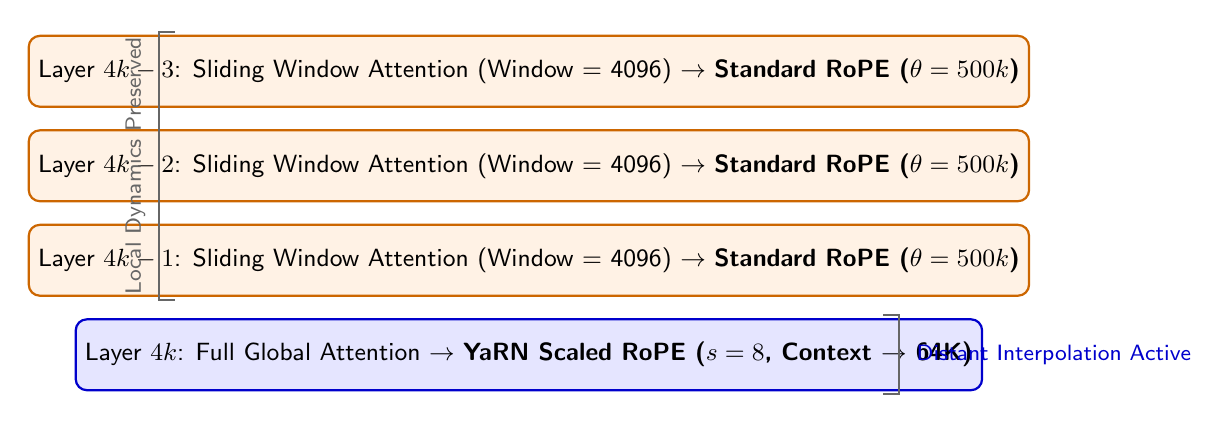
\begin{tikzpicture}[
    layer_swa/.style={draw=orange!80!black, fill=orange!10, rounded corners=4pt, font=\small\sffamily, align=center, thick},
    layer_full/.style={draw=blue!80!black, fill=blue!10, rounded corners=4pt, font=\small\sffamily, align=center, thick},
    bracket/.style={thick, color=gray!80!black}
]
    \node[layer_swa, minimum width=8.5cm, minimum height=0.9cm] (l1) at (0, 3.6) {Layer $4k-3$: Sliding Window Attention (Window = 4096) $\to$ \textbf{Standard RoPE ($\theta = 500\text{k}$)}};
    \node[layer_swa, minimum width=8.5cm, minimum height=0.9cm] (l2) at (0, 2.4) {Layer $4k-2$: Sliding Window Attention (Window = 4096) $\to$ \textbf{Standard RoPE ($\theta = 500\text{k}$)}};
    \node[layer_swa, minimum width=8.5cm, minimum height=0.9cm] (l3) at (0, 1.2) {Layer $4k-1$: Sliding Window Attention (Window = 4096) $\to$ \textbf{Standard RoPE ($\theta = 500\text{k}$)}};
    \node[layer_full, minimum width=8.5cm, minimum height=0.9cm] (l4) at (0, 0.0) {Layer $4k$: Full Global Attention $\to$ \textbf{YaRN Scaled RoPE ($s = 8$, Context $\to$ 64K)}};
    
    \draw[bracket] (-4.5, 4.1) -- (-4.7, 4.1) -- (-4.7, 0.7) -- (-4.5, 0.7);
    \node[font=\footnotesize\sffamily, rotate=90, text=gray!80!black] at (-5.0, 2.4) {Local Dynamics Preserved};

    \draw[bracket] (4.5, 0.5) -- (4.7, 0.5) -- (4.7, -0.5) -- (4.5, -0.5);
    \node[font=\footnotesize\sffamily, text=blue!80!black, right] at (4.8, 0.0) {Distant Interpolation Active};
\end{tikzpicture}
\end{center}
\end{latin}